% Author: Nelson Lago
% This file is distributed under the MIT Licence

%%%%%%%%%%%%%%%%%%%%%%%%%%%%%%%%%%%%%%%%%%%%%%%%%%%%%%%%%%%%%%%%%%%%%%%%%%%%%%%%
%%%%%%%%%%%%%%%%%%%%%%%%%%%%%%%%% PREÂMBULO %%%%%%%%%%%%%%%%%%%%%%%%%%%%%%%%%%%%
%%%%%%%%%%%%%%%%%%%%%%%%%%%%%%%%%%%%%%%%%%%%%%%%%%%%%%%%%%%%%%%%%%%%%%%%%%%%%%%%

% A língua padrão é a última da lista
\documentclass[a1paper,brazilian,english]{article}

% Vários pacotes e opções de configuração genéricos
\usepackage{imegoodies}
\usepackage[poster,hidelinks]{imelooks}
\tcbposterset{fontsize = 30pt} % default, mude se necessário

% Diretórios onde estão as figuras; com isso, não é necessário (mas
% é permitido) colocar o caminho completo em \includegraphics. Note
% que a extensão nunca é necessária (mas é permitida), ou seja, o
% resultado é o mesmo com "\includegraphics{figuras/foto.jpeg}",
% "\includegraphics{foto.jpeg}", "\includegraphics{figuras/foto}"
% ou "\includegraphics{foto}".
\graphicspath{{figuras/},{fig/},{logos/},{img/},{images/},{imagens/}}

% Comandos rápidos para mudar de língua:
% \en -> muda para o inglês
% \br -> muda para o português
% \texten{blah} -> o texto "blah" é em inglês
% \textbr{blah} -> o texto "blah" é em português
\babeltags{br = brazilian, en = english}


%%%%%%%%%%%%%%%%%%%%%%%%%%%%%%%%%%%%%%%%%%%%%%%%%%%%%%%%%%%%%%%%%%%%%%%%%%%%%%%%
%%%%%%%%%%%%%%%%%%%%%%%%%%%%%%%%%% METADADOS %%%%%%%%%%%%%%%%%%%%%%%%%%%%%%%%%%%
%%%%%%%%%%%%%%%%%%%%%%%%%%%%%%%%%%%%%%%%%%%%%%%%%%%%%%%%%%%%%%%%%%%%%%%%%%%%%%%%

% O arquivo com os dados bibliográficos para biblatex; você pode usar
% este comando mais de uma vez para acrescentar múltiplos arquivos
\addbibresource{bibliografia.bib}

% Este comando permite acrescentar itens à lista de referências sem incluir
% uma referência de fato no texto (pode ser usado em qualquer lugar do texto)
%\nocite{bronevetsky02,schmidt03:MSc, FSF:GNU-GPL, CORBA:spec, MenaChalco08}
% Com este comando, todos os itens do arquivo .bib são incluídos na lista
% de referências
%\nocite{*}


%%%%%%%%%%%%%%%%%%%%%%%%%%%%%%%%%%%%%%%%%%%%%%%%%%%%%%%%%%%%%%%%%%%%%%%%%%%%%%%%
%%%%%%%%%%%%%%%%%%%%%%%%%%%%%%% INÍCIO DO POSTER %%%%%%%%%%%%%%%%%%%%%%%%%%%%%%%
%%%%%%%%%%%%%%%%%%%%%%%%%%%%%%%%%%%%%%%%%%%%%%%%%%%%%%%%%%%%%%%%%%%%%%%%%%%%%%%%


% Existem várias packages para criar pôsteres com LaTeX (a0poster, baposter,
% tikzposter, sciposter...). As mais comuns atualmente são beamerposter
% e tcolorbox (com sua biblioteca "poster"). Ambas funcionam muito bem;
% beamerposter é mais familiar (ela simplesmente utiliza beamer com alguns
% ajustes no tamanho das fontes e do papel), mas com tcolorbox o alinhamento
% vertical dos elementos é MUITO mais simples, e esta é a solução adotada
% aqui. Vale muito a pena ler a documentação com "texdoc tcolorbox" e
% "texdoc tcolorbox-tutorial-poster".

% Um pôster com tcolorbox é composto por blocos (posterboxes) coloridos
% de tamanho variável; cada bloco pode conter textos ou imagens e um
% título opcional. O pôster utiliza uma grade de dimensões definidas em
% \begin{tcposter} com "rows=" e "columns=" para fazer o alinhamento:
% para cada posterbox, podemos dizer "row=X, column=Y" para definir sua
% posição. Além disso, podemos dizer "span=A, rowspan=B" para fixar
% seu tamanho. Sem "span" e "rowspan", uma posterbox tem pelo menos o
% tamanho de uma célula da grade, mas se seu tamanho natural for maior
% ela extrapola esse tamanho. "span" e "rowspan" podem ser números
% não-inteiros (como 0.8 ou 1.4).
%
% "\begin{posterbox}" recebe um conjunto de parâmetros opcional e um
% conjunto de parâmetros obrigatório:
%
% "\begin{posterbox}[opcional]{obrigatório}".
%
% O conjunto de parâmetros opcional é onde inserimos os parâmetros comuns
% de tcolorbox, como "adjusted title", "coltext", "titlerule" etc.; o
% conjunto de parâmetros obrigatório é usado para determinar as dimensões
% e a posição da posterbox, ou seja, as opções "name", "column", "below",
% "span" etc.
%
% ALINHAMENTO HORIZONTAL
%
% É possível definir um poster com 2 colunas e fazer algo como
%
% \posterbox{column=1, span=1.3}{blah}
% \posterbox{column*=2, span=0.7}{blah}
%
% A segunda posterbox será alinhada à direita ("column*="), então as
% duas serão colocadas lado-a-lado sem sobreposições.
%
% Na prática, no entanto, é mais fácil fazer como no exemplo abaixo:
% definimos que o poster tem 12 colunas, o que nos permite dividir
% sua largura em 2, 3, 4 ou 6 colunas iguais ou diferentes (como
% 1/2 + 1/2, 2/3 + 1/3, 1/4 + 1/4 + 1/2, 1/4 + 1/6 + 1/4 + 1/3 etc).
%
% ALINHAMENTO VERTICAL
%
% Embora seja possível alinhar as posterboxes em função da grade na
% vertical, uma outra possibilidade é utilizar "above", "below" e
% "between", como no exemplo abaixo: basta associar um nome "blah" a
% uma determinada posterbox e, em outra, dizer "below=blah". Lembre-se
% que a posterbox de nome "blah" deve ser definida *antes* que outra
% possa fazer referência a ela. Também é possível fazer "below=top",
% "above=bottom" etc. A opção "equal height group" também é muito útil.
% Nada impede que você use estratégias de alinhamento diferentes para
% cada posterbox.

% Este modelo define a opção "smallmargins", que diminui a distância
% entre o conteúdo de uma posterbox e suas bordas. Use com parcimônia!


\newcommand{\rfsigma}{\mathbb{R}\mathcal{F}^\sigma}
\newcommand{\asigma}{\mathcal{A}^\sigma}

\newcommand{\emptyflag}{\varnothing}
\newcommand{\isom}{\cong}

% Tikz setup from https://arxiv.org/abs/2103.14179


\newcommand{\vc}[1]{\ensuremath{\vcenter{\hbox{#1}}}}
\tikzset{vtx/.style={inner sep=1.7pt, outer sep=0pt, circle, fill}}
\tikzset{unlabeled_vertex/.style={inner sep=1.7pt, outer sep=0pt, circle, fill, draw=black}}
\tikzset{labeled_vertex/.style={inner sep=2.2pt, outer sep=0pt, rectangle, fill=yellow, draw=black}}
\tikzset{edge_color0/.style={color=black,line width=1.2pt}}
\tikzset{edge_color1/.style={color=red,  line width=1.2pt,opacity=0}}
\tikzset{edge_color2/.style={color=blue, line width=1.2pt,opacity=1}}

\newcommand{\flagone}{ % this is the unlabeled triangle
  \vc{
\begin{tikzpicture}[scale=0.5]
    \draw \foreach \x in {0,1,2}{(270+\x*360/3:0.8) coordinate(x\x)};
    \draw[edge_color2] (x0)--(x1)--(x2)--(x0);
    \draw (x0) node[unlabeled_vertex]{};
    \draw (x1) node[unlabeled_vertex]{};
    \draw (x2) node[unlabeled_vertex]{};
  \end{tikzpicture}}
}
\newcommand{\kthree}{\flagone}

\newcommand{\flagtwo}{ % this is the unlabeled edge
  \vc{
\begin{tikzpicture}[scale=0.5]
    \draw (225:0.8) coordinate(x0);
    \draw (45:0.8) coordinate(x1);
    \draw[edge_color2] (x0)--(x1);
    \draw (x0) node[unlabeled_vertex]{};
    \draw (x1) node[unlabeled_vertex]{};
  \end{tikzpicture}}
}
\newcommand{\edge}{\flagtwo}

\newcommand{\flagthree}{ % this represents the edges among non-neighbors of a vertex
  \vc{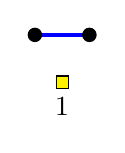
\begin{tikzpicture}[scale=0.5]
    \draw \foreach \x in {0,1,2}{(270+\x*360/3:0.8) coordinate(x\x)};
    \draw[edge_color2] (x1)--(x2);
    \draw (x0) node[labeled_vertex,label=below:$1$]{};
    \draw (x1) node[unlabeled_vertex]{};
    \draw (x2) node[unlabeled_vertex]{};
  \end{tikzpicture}}
}

\newcommand{\flagfour}{
  \vc{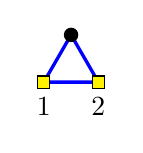
\begin{tikzpicture}[scale=0.5]
    \draw \foreach \x in {0,1,2}{(210+\x*360/3:0.8) coordinate(x\x)};
    \draw[edge_color2] (x0)--(x1)--(x2)--(x0);
    \draw (x0) node[labeled_vertex,label=below:$1$]{};
    \draw (x1) node[labeled_vertex,label=below:$2$]{};
    \draw (x2) node[unlabeled_vertex]{};
  \end{tikzpicture}}
}
\newcommand{\kthreeLabeledEdge}{\flagfour}

\newcommand{\flagfive}{ % this is the labeled edge
  \vc{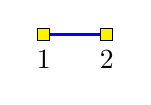
\begin{tikzpicture}[scale=0.5]
    \draw (180:0.8) coordinate(x0);
    \draw (360:0.8) coordinate(x1);
    \draw[edge_color2] (x0)--(x1);
    \draw (x0) node[labeled_vertex,label=below:$1$]{};
    \draw (x1) node[labeled_vertex,label=below:$2$]{};
  \end{tikzpicture}}
}
\newcommand{\labeledEdge}{\flagfive}

\newcommand{\flagsix}{ % this is the labeled non-edge
  \vc{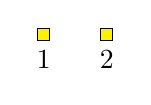
\begin{tikzpicture}[scale=0.5]
    \draw (180:0.8) coordinate(x0);
    \draw (360:0.8) coordinate(x1);
    \draw (x0) node[labeled_vertex,label=below:$1$]{};
    \draw (x1) node[labeled_vertex,label=below:$2$]{};
  \end{tikzpicture}}
}
\newcommand{\labeledNonEdge}{\flagsix}

\newcommand{\flagseven}{
  \vc{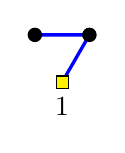
\begin{tikzpicture}[scale=0.5]
    \draw \foreach \x in {0,1,2}{(270+\x*360/3:0.8) coordinate(x\x)};
    \draw[edge_color2] (x0)--(x1)--(x2);
    \draw (x0) node[labeled_vertex,label=below:$1$]{};
    \draw (x1) node[unlabeled_vertex]{};
    \draw (x2) node[unlabeled_vertex]{};
  \end{tikzpicture}}
}

\newcommand{\flageight}{ % this is the labeled edge with an extra vertex joined to 1
  \vc{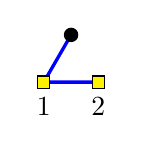
\begin{tikzpicture}[scale=0.5]
    \draw \foreach \x in {0,1,2}{(210+\x*360/3:0.8) coordinate(x\x)};
    \draw[edge_color2] (x2)--(x0)--(x1);
    \draw (x0) node[labeled_vertex,label=below:$1$]{};
    \draw (x1) node[labeled_vertex,label=below:$2$]{};
    \draw (x2) node[unlabeled_vertex]{};
  \end{tikzpicture}}
}

\newcommand{\flagnine}{ % this is the labeled edge with an extra vertex joined to 2
  \vc{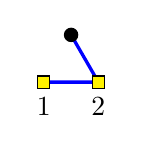
\begin{tikzpicture}[scale=0.5]
    \draw \foreach \x in {0,1,2}{(210+\x*360/3:0.8) coordinate(x\x)};
    \draw[edge_color2] (x0)--(x1)--(x2);
    \draw (x0) node[labeled_vertex,label=below:$1$]{};
    \draw (x1) node[labeled_vertex,label=below:$2$]{};
    \draw (x2) node[unlabeled_vertex]{};
  \end{tikzpicture}}
}

\newcommand{\flagten}{
  \vc{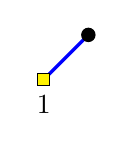
\begin{tikzpicture}[scale=0.5]
    \draw (225:0.8) coordinate(x0);
    \draw (45:0.8) coordinate(x1);
    \draw[edge_color2] (x0)--(x1);
    \draw (x0) node[labeled_vertex,label=below:$1$]{};
    \draw (x1) node[unlabeled_vertex]{};
  \end{tikzpicture}}
}
\newcommand{\edgeWithOneLabel}{\flagten}

\newcommand{\flageleven}{
  \vc{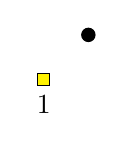
\begin{tikzpicture}[scale=0.5]
    \draw (225:0.8) coordinate(x0);
    \draw (45:0.8) coordinate(x1);
    \draw (x0) node[labeled_vertex,label=below:$1$]{};
    \draw (x1) node[unlabeled_vertex]{};
  \end{tikzpicture}}
}
\newcommand{\nonEdgeWithOneLabel}{\flageleven}

\newcommand{\flagtwelve}{
  \vc{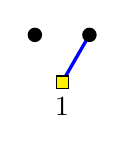
\begin{tikzpicture}[scale=0.5]
    \draw \foreach \x in {0,1,2}{(270+\x*360/3:0.8) coordinate(x\x)};
    \draw[edge_color2] (x0)--(x1);
    \draw (x0) node[labeled_vertex,label=below:$1$]{};
    \draw (x1) node[unlabeled_vertex]{};
    \draw (x2) node[unlabeled_vertex]{};
  \end{tikzpicture}}
}

\begin{document}

% Em um poster não há \maketitle

\begin{tcbposter}[
  poster = {
    %showframe, % muito útil durante a preparação do poster
    rows = 6,
    columns = 12,
    colspacing = 1.2cm,
    rowspacing = .8cm,
  },
]


\posterbox[titlebox]{name=titlebox, below=top, column=1, span=12}{
    Sobre uma conjectura de Erd\H os acerca de grafos livres de triângulos
}

\posterbox[footerbox]{name=footerbox, above=bottom, column=1, span=12}{
    \large
    Aluno: Marcelo Machado Lage\par
    \vspace{4pt}
    \large
    Orientador: Prof.~Dr.~Guilherme Oliveira Mota\par
    \vspace{4pt}
    \small
    \textcolor{imesoftblue!30!white}
      {Departmento de Ciência da Computação --- Instituto de Matemática e Estatística --- Universidade de São Paulo}\\
    \small    
    \textit{Durante a realização desse projeto, o aluno recebeu apoio da FAPESP. Processos nº 2025/06707-6, 2025/14743-2.}\relax
}

\posterbox[adjusted title=Referências]{name=refbox, column=5, span=8, above=footerbox}{
  \begin{enumerate}[label={[\arabic*]}]
    \item\label{EFPS} Erd\H os, Faudree et. al.. \textit{How to Make a Graph Bipartite. (1988)}
    \item\label{BCL} Balogh et. al. \textit{Max cuts in triangle-free graphs. (2021)}
    \item\label{CJK} Chen et. al. \textit{Triangle-free graphs with large degree. (1997)}
\end{enumerate}
}

\posterbox[adjusted title=Introdução e motivação]{name=introbox, column=1, span=4, below=titlebox}{
  Um grafo $G$ é um par $(V,E)$, onde $V$ são os \emph{vértices} e $E$ são as \emph{arestas} (pares não ordenados de vértices).
  A Teoria Extremal dos Grafos estuda propriedades de grafos sob restrições estruturais. Compreender propriedades extremais tem aplicações em análise de algoritmos, modelagem de redes e otimização.
  
  \begin{itemize}
    \item Grafos livres de triângulos não contêm ciclos de tamanho $3$.
    \item Pergunta natural: quantas arestas um grafo livre de triângulos pode ter?
    \item \textbf{Teorema de Mantel.} Um grafo com $n$ vértices sem triângulos possui no máximo $\left\lfloor\frac{n^2}{4}\right\rfloor$ arestas.
  \end{itemize}
}

\posterbox[adjusted title=Problema e objetivos]{name=problembox, column=1, span=4, between=introbox and footerbox}{
  Os únicos grafos que satisfazem igualdade no Teorema de Mantel são bipartidos.
  \begin{itemize}
    \item Pergunta natural: quão ``distante'' pode estar um grafo sem triângulos de um bipartido?
    %\item Grafos pouco densos são quase bipartidos pois o grafo vazio é bipartido; grafos muito densos são quase bipartidos porque o exemplo extremal de Mantel é bipartido.
    \item $D(G)$ mede essa distância pela remoção de um menor conjunto de arestas que torna $G$ bipartido.
  \end{itemize}
  \textbf{Conjectura 1 (Erd\H os, 1975).} Todo grafo livre de triângulos $G$ com $n$ vértices satisfaz $D(G) \leq \frac{n^2}{25}$.

  O caso geral da Conjectura 1 permanece em aberto.

  \centering
  \begin{figure}[H]
    \include{figuras/c5-blowup-tikz}
    \caption*{O blow-up de $C_5$ em que cada classe tem $\frac{n}{5}$ vértices satisfaz $e(G)=\frac{n^2}{5}$ e $D(G)=\frac{n^2}{25}$.}
  \end{figure}
}



\posterbox[adjusted title=Metodologia]{name=methodbox, column=5, span=8, below=titlebox}{
  \begin{itemize}
    \item Álgebras de flag\\$\rightarrow$ traduzem problemas de densidade em programas semidefinidos.
    \item Blow-ups\\$\rightarrow$ expandem vértices para conjuntos independentes mantendo estrutura.
    \item Condições de grau mínimo\\$\rightarrow$ permitem simplificar o problema para blow-ups de grafos pequenos.
  \end{itemize}
}


\posterbox[adjusted title=Resultados principais]{name=resultbox, column=5, span=8, below=methodbox}{
    \begin{itemize}
      \item \textit{(Simonovits 1968)} $\rightarrow$ Se $e(G) = \frac{n^2}{4}-m$, então $D(G) \leq m$.
        \begin{itemize}
          \item Resolve a Conjectura 1 se $e(G) \geq 0.21n^2$.
        \end{itemize}
      \item \ref{EFPS} $\rightarrow$ Prova de $D(G) \leq \frac{4e(G)^2}{n^2}$ e $D(G) \leq \frac{n^2}{18+\epsilon}$ (para algum $\epsilon>0$).
        \begin{itemize}
          \item Cota explícita sobre $D(G)$; resolve a Conjectura 1 se $e(G) \geq \frac{n^2}{5} = 0.20n^2$.
        \end{itemize}
      \item \ref{BCL} $\rightarrow$ Generaliza~\ref{EFPS}: prova a Conjectura 1 se $e(G) \geq 0.159n^2$ e outros resultados parciais usando \emph{álgebras de flag}.
      \item A Conjectura 1 também pode ser resolvida quando $\delta(G) \geq \frac{4n}{11}$ usando~\ref{CJK}.
    \end{itemize}

    \centering
    \begin{figure}[H]
      \begin{subfigure}[c]{.48\textwidth}
        \centering
        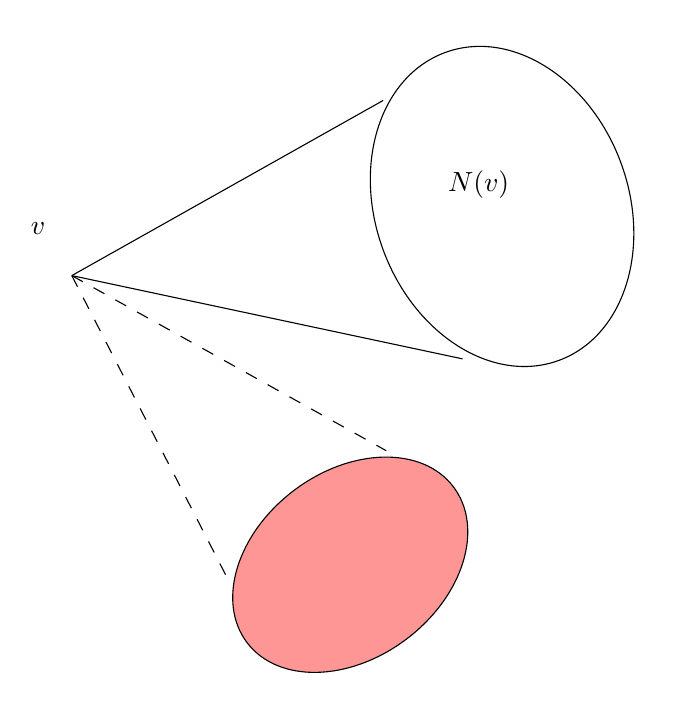
\begin{tikzpicture}[x=0.75pt,y=0.75pt,yscale=-1,xscale=1,scale=1.5]
%uncomment if require: \path (0,300); %set diagram left start at 0, and has height of 300

%Straight Lines [id:da9079454219601542] 
\draw    (70,147) -- (195.5,173.75) ;
%Straight Lines [id:da01422580791198047] 
\draw    (70,147) -- (170,90.75) ;
%Shape: Ellipse [id:dp6541371174832803] 
\draw   (189.83,75.38) .. controls (210.88,67.55) and (236.17,83.33) .. (246.31,110.62) .. controls (256.46,137.91) and (247.61,166.37) .. (226.56,174.2) .. controls (205.51,182.02) and (180.22,166.24) .. (170.08,138.96) .. controls (159.94,111.67) and (168.78,83.2) .. (189.83,75.38) -- cycle ;
%Shape: Ellipse [id:dp4716129095851628] 
\draw  [color={rgb, 255:red, 0; green, 0; blue, 0 }  ,draw opacity=1 ][fill={rgb, 255:red, 255; green, 150; blue, 150 }  ,fill opacity=1 ] (192.61,214.9) .. controls (202.55,228.12) and (195.76,250.01) .. (177.43,263.8) .. controls (159.11,277.59) and (136.19,278.05) .. (126.25,264.84) .. controls (116.31,251.62) and (123.1,229.73) .. (141.43,215.95) .. controls (159.75,202.16) and (182.67,201.69) .. (192.61,214.9) -- cycle ;
%Straight Lines [id:da2703367837180948] 
\draw  [dash pattern={on 4.5pt off 4.5pt}]  (70,147) -- (120,244.25) ;
%Straight Lines [id:da985102390949472] 
\draw  [dash pattern={on 4.5pt off 4.5pt}]  (70,147) -- (171,203.25) ;

% Text Node
\draw (56,129) node [anchor=north west][inner sep=0.75pt]   [align=left] {$\displaystyle v$};
% Text Node
\draw (190,112.5) node [anchor=north west][inner sep=0.75pt]   [align=left] {$\displaystyle N( v)$};


\end{tikzpicture}

        \caption*{Observe que~$\textstyle{D(G) \leq e(G-N(v))}$.
        Na linguagem de álgebras de flag, essa figura representa o corte local gerado relacionado à restrição $\average{\labeledCherryComplement} \geq \frac{2}{25}$.}
      \end{subfigure}
      \hfill
      \begin{subfigure}[c]{.48\textwidth}
        \centering
        \tikzset{
    % Define a style called "my_line_style" that uses 'line width=2pt'
    my_line_style/.style={line width=7pt} 
}

\begin{tikzpicture}[x=0.75pt,y=0.75pt,yscale=-1,xscale=1]
%uncomment if require: \path (0,300); %set diagram left start at 0, and has height of 300

%Straight Lines [id:da5581831139118527] 
\draw[my_line_style]    (126.85,62.85) -- (295.15,231.15) ;
%Straight Lines [id:da5995296745227333] 
\draw[my_line_style]    (92,147) -- (330,147) ;
%Straight Lines [id:da3040978363517214] 
\draw[my_line_style]    (126.85,231.15) -- (295.15,62.85) ;
%Straight Lines [id:da9046950317683012] 
\draw[my_line_style]    (211,266) -- (211,28) ;
%Straight Lines [id:da2329743835242285] 
\draw[my_line_style]    (211,266) -- (126.85,62.85) ;
%Straight Lines [id:da2555941663960718] 
\draw[my_line_style]    (330,147) -- (126.85,62.85) ;
%Straight Lines [id:da7186386958802977] 
\draw[my_line_style]    (295.15,231.15) -- (92,147) ;
%Straight Lines [id:da717843693102989] 
\draw[my_line_style]    (295.15,62.85) -- (92,147) ;
%Straight Lines [id:da549150945626202] 
\draw[my_line_style]    (330,147) -- (126.85,231.15) ;
%Straight Lines [id:da32971398522152695] 
\draw[my_line_style]    (211,266) -- (295.15,62.85) ;
%Straight Lines [id:da7444985407616169] 
\draw[my_line_style]    (126.85,231.15) -- (211,28) ;
%Straight Lines [id:da9205588924423223] 
\draw[my_line_style]    (211,28) -- (295.15,231.15) ;
%Shape: Circle [id:dp42856305661994043] 
\draw  [fill={rgb, 255:red, 255; green, 255; blue, 255 }  ,fill opacity=1 ] (52.81,147) .. controls (52.81,125.36) and (70.36,107.81) .. (92,107.81) .. controls (113.64,107.81) and (131.19,125.36) .. (131.19,147) .. controls (131.19,168.64) and (113.64,186.19) .. (92,186.19) .. controls (70.36,186.19) and (52.81,168.64) .. (52.81,147) -- cycle ;
%Shape: Circle [id:dp5422329348821533] 
\draw  [fill={rgb, 255:red, 255; green, 255; blue, 255 }  ,fill opacity=1 ] (105.43,231.15) .. controls (105.43,219.31) and (115.02,209.72) .. (126.85,209.72) .. controls (138.69,209.72) and (148.28,219.31) .. (148.28,231.15) .. controls (148.28,242.98) and (138.69,252.57) .. (126.85,252.57) .. controls (115.02,252.57) and (105.43,242.98) .. (105.43,231.15) -- cycle ;
%Shape: Circle [id:dp07099123559615339] 
\draw  [fill={rgb, 255:red, 255; green, 255; blue, 255 }  ,fill opacity=1 ] (183.61,266) .. controls (183.61,250.87) and (195.87,238.61) .. (211,238.61) .. controls (226.13,238.61) and (238.39,250.87) .. (238.39,266) .. controls (238.39,281.13) and (226.13,293.39) .. (211,293.39) .. controls (195.87,293.39) and (183.61,281.13) .. (183.61,266) -- cycle ;
%Shape: Circle [id:dp5622234814824223] 
\draw  [fill={rgb, 255:red, 255; green, 255; blue, 255 }  ,fill opacity=1 ] (263.03,231.15) .. controls (263.03,213.41) and (277.41,199.03) .. (295.15,199.03) .. controls (312.89,199.03) and (327.27,213.41) .. (327.27,231.15) .. controls (327.27,248.89) and (312.89,263.27) .. (295.15,263.27) .. controls (277.41,263.27) and (263.03,248.89) .. (263.03,231.15) -- cycle ;
%Shape: Circle [id:dp99639590204173] 
\draw  [fill={rgb, 255:red, 255; green, 255; blue, 255 }  ,fill opacity=1 ] (301.95,147) .. controls (301.95,131.51) and (314.51,118.95) .. (330,118.95) .. controls (345.49,118.95) and (358.05,131.51) .. (358.05,147) .. controls (358.05,162.49) and (345.49,175.05) .. (330,175.05) .. controls (314.51,175.05) and (301.95,162.49) .. (301.95,147) -- cycle ;
%Shape: Circle [id:dp42018330238360857] 
\draw  [fill={rgb, 255:red, 255; green, 255; blue, 255 }  ,fill opacity=1 ] (254.05,62.85) .. controls (254.05,40.16) and (272.45,21.76) .. (295.15,21.76) .. controls (317.84,21.76) and (336.24,40.16) .. (336.24,62.85) .. controls (336.24,85.55) and (317.84,103.95) .. (295.15,103.95) .. controls (272.45,103.95) and (254.05,85.55) .. (254.05,62.85) -- cycle ;
%Shape: Circle [id:dp781256081687053] 
\draw  [fill={rgb, 255:red, 255; green, 255; blue, 255 }  ,fill opacity=1 ] (190.83,28) .. controls (190.83,16.86) and (199.86,7.83) .. (211,7.83) .. controls (222.14,7.83) and (231.17,16.86) .. (231.17,28) .. controls (231.17,39.14) and (222.14,48.17) .. (211,48.17) .. controls (199.86,48.17) and (190.83,39.14) .. (190.83,28) -- cycle ;
%Shape: Circle [id:dp9871521798304426] 
\draw  [fill={rgb, 255:red, 255; green, 255; blue, 255 }  ,fill opacity=1 ] (101.85,62.85) .. controls (101.85,49.05) and (113.05,37.85) .. (126.85,37.85) .. controls (140.66,37.85) and (151.85,49.05) .. (151.85,62.85) .. controls (151.85,76.66) and (140.66,87.85) .. (126.85,87.85) .. controls (113.05,87.85) and (101.85,76.66) .. (101.85,62.85) -- cycle ;




\end{tikzpicture}
        \caption*{Se~$\textstyle{\delta(G) \geq \frac{4n}{11}}$, então $G$ é da forma acima, e é possível demonstrar a Conjectura 1 usando essa informação estrutural extra.}
      \end{subfigure}
    \end{figure}
}


\posterbox[adjusted title=Discussão]{name=discussbox, column=5, span=4.5, between=resultbox and refbox}{
  \begin{itemize}
    \item As cotas conhecidas funcionam melhor para grafos densos: resultados do tipo ``a Conjectura 1 vale se $e(G) \geq \alpha n^2$'';
    \item Uso de álgebras de flag fornece desigualdades assintóticas a partir de otimização (numérico);
    \item Condições de grau mínimo permite simplificação estrutural e estudo da Conjectura 1 para certos grafos abaixo do limiar $e(G) \geq \frac{n^2}{5}$ (estrutural).
  \end{itemize}
}

\posterbox[adjusted title=Conclusão]{name=conclusionbox, column*=12, span=3.5, between=resultbox and refbox}{
  O uso de álgebras de flag e condições de grau mínimo confirmam a Conjectura 1 em subclasses de grafos densos.
  O trabalho contribui revisando os métodos usados no problema e com uma prova alternativa para o caso $\delta(G) > \frac{4n}{11}$.
}











\end{tcbposter}

\end{document}
